\documentclass[11pt,a4paper,english]{article}
\usepackage{natbib}  % Adds support for different citation styles
\bibliographystyle{chicago}
\usepackage[T1]{fontenc}
\usepackage[utf8]{inputenc}
\usepackage{babel}
\usepackage{blindtext}
\usepackage[nodayofweek,level]{datetime}
\newdate{date}{25}{03}{2025}
\date{\displaydate{date}}
\usepackage[a4paper,margin=1in]{geometry}
\usepackage{graphicx}
\usepackage{setspace}
\usepackage{amsmath}
\usepackage{hyperref}
\usepackage{tabularx}
\usepackage{booktabs}
\doublespacing



\title{Building Efficient Portfolios
\thanks{Code and data supporting this analysis is available at: \url{https://github.com/Aman-Rana-02/Efficient_Market_Portfolios}}}
\author{%
  Aman Rana\\
  \small Department of Computer Science\\
  \small University of Toronto\\
  \small\texttt{aman.rana@mail.utoronto.ca}
}

\begin{document}
  \maketitle

  \begin{abstract}
    \noindent This article provides a brief and accessible overview of three fundamental concepts in modern portfolio theory: the Capital Asset Pricing Model (CAPM), Markowitz Mean-Variance Optimization (MVO), and Arbitrage Pricing Theory (APT). 
    We begin by exploring the CAPM, which describes the relationship between systematic risk and expected return for assets, particularly stocks. 
    Next, we delve into Markowitz MVO, a framework for assembling a portfolio of assets such that the expected return is maximized for a given level of risk, using this to build the efficient frontier.
     Finally, we examine APT, which extends the ideas of CAPM by considering multiple factors that might affect asset returns.
     We conclude by discussing the advantages and limitations of these models.
  \end{abstract}

  \newpage
  \tableofcontents

  \newpage

  \section{Introduction}
\label{sec:introduction}
TODO the INTRO!!!!!

The remainder of the article is structured as follows:
\begin{itemize}
    \item Section~\ref{sec:data} provides an overview of the dataset used for analysis.
    \item Section~\ref{sec:capital_asset_pricing_model} explores the Capital Asset Pricing Model (CAPM) and its implications.
    \item Section~\ref{sec:diversification_and_portfolios} discusses the importance of diversification and the construction of efficient portfolios.
    \item Section~\ref{sec:arbitrage_pricing_theory} delves into the Arbitrage Pricing Theory (APT) and its applications.
    \item Section~\ref{sec:conclusion} concludes by discussing limitations of the methods discussed.
\end{itemize}

  \section{Data}
\label{sec:data}
% Description of the dataset used for analysis
We use Python \citep{python3}, Pandas \citep{reback2020pandas}, NumPy \citep{harris2020array}, Statsmodels \citep{seabold2010statsmodels} to analyze S\&P 500 price data from Finaeon's Global Financial Dataset \citep{finaeon} and the Fama-French 3-factor data library \citep{french_website}. 
We use Matplotlib for plotting \citep{Hunter2007}.
We get the S\&P500's current constituents from the Finaeon website, and download a time-series of daily prices for each stock using Finaeon's API. 
Kenneth french's website \citep{french_website} provides the risk-free rate, market excess return, and daily returns of the Size and Value portfolios. 
The risk-free rate they provide is the 1-month T-bill rate, and the market risk premium is the difference between the total US stock market's return and the risk-free rate.
The size and value portfolios are constructed according to \citet{fama_french_1993}.
By only using the return histories of the current S\&P 500 constituents, we introduce a survivorship bias in our analysis. Any risk premia we include will be biased upwards, as we only consider firms that have survived to the present day.
The purpose of this article is to introduce concepts of modern portfolio theory, and not to provide a comprehensive analysis of risk factors and premia, so we
note this deficiency and move forward with our analysis.

\begin{table}
    \centering
    \begin{tabular}{|c|c|c|}
        \hline
        \textbf{Company Name} & \textbf{Ticker}\\
        \hline
        Apple Inc. & AAPL\\
        General Electric Co. & GE\\
        International Business Machines Corp. & IBM\\
        The Coca-Cola Company & KO\\
        Microsoft Corp. & MSFT\\
        \hline
    \end{tabular}
    \caption{Sample assets and their full names}
    \label{tab:sample_assets_w_names}
\end{table}

Throughout this article, we'll use a few sample assets to illustrate concepts. We'll refer to them by ticker symbol, and their full names are shown in table \ref{tab:sample_assets_w_names}.
These are randomly chosen from the S\&P 500, and are not meant to be representative of the index as a whole.

% #TODO: Show a snippet of the data. Mention any windsorizing.
 
  \section{Capital Asset Pricing Model (CAPM)}
\label{sec:capital_asset_pricing_model}

\subsection{Intuition of the CAPM \texorpdfstring{$\beta$}{beta}}
\begin{equation}
    \label{eq:capm}
    E[R_i] = R_f + \beta_i (E[R_m] - R_f)
\end{equation}

The Capital Asset Pricing Model is a model that describes the expected returns of an asset as a function of its exposure to systematic risk.
The model is given by Equation \ref{eq:capm}, where:
\begin{itemize}
    \item $E[R_i]$ is the expected return of asset $i$
    \item $R_f$ is the risk-free rate
    \item $\beta_i$ is the asset's beta
    \item $E[R_m]$ is the expected return of the market
\end{itemize}

Notice that according to the model, a firm's expected return is only a function of its expsure to the market's risk.
This comes from a fundamental belief that in the long-run, any firm-specific/idiosyncratic risk can be diversified away, therefore
investors look to be compensated for the risk that cannot be diversified away, which is the market risk.

To estimate the CAPM beta for firms, we regress a firm's historical returns against the market's returns, and take the slope of the line of best fit.
This is given by Equation \ref{eq:beta_regression}:
\begin{equation}
    \label{eq:beta_regression}
    R_i - R_f = \alpha + \beta_i (R_m - R_f) + \epsilon
\end{equation}

Where:
\begin{itemize}
    \item $R_i$ is the firm's return
    \item $R_f$ is the risk-free rate
    \item $R_m$ is the market return
    \item $\alpha$ is the intercept of the regression line
    \item $\beta_i$ is the slope of the regression line
    \item $\epsilon$ is the error term
\end{itemize}

$\alpha$ is known as Jensen's alpha, it is a reflection of how much a firm under or outperforms the market, given its beta.
In a world where CAPM perfectly models a firm's returns, $\alpha$ should be zero.

\begin{table}
    \centering
    \begin{tabular}{|c|c|c|}
        \hline
        \textbf{Asset} & \textbf{Beta}\\
        \hline
        AAPL & 1.10\\
        GE & 0.92\\
        IBM & 0.75\\
        KO & 0.49\\
        MSFT & 1.14\\
        \hline
    \end{tabular}
    \caption{Sample assets and their CAPM betas}
    \label{tab:sample_assets_capm}
\end{table}

Table \ref{tab:sample_assets_capm} shows the CAPM betas for a few sample assets. Higher beta assets are 'riskier' since they are more 
exposed to the market's risk, and therefore should have higher expected returns.

We can see this more clearly in figure \ref{fig:historical_expected_returns_vs_beta}, where we plot the historical 
average annualized return against a firm's beta. We can see that there is a positive relationship between beta and expected return.

\subsection{Cost of Capital - DDM vs CAPM}
% Explain the cost of capital
% Explain how to calculate it using the DDM
% Explain how to calculate it using the CAPM
% Explain the fundamental intuition of the difference between the two

Recall the definition of cost of capital, and that it is synonymous with expected return.
We previously explored using the Dividend Discount Model (DDM) to estimate the cost of capital. The intuition of the 
DDM is that a stock price represents the present value of all future cashflows, where we proxy all future cashflows using a dividend and expected growth rate.
A DDM feels more realistic the better we can forecast a firm's future dividends, as well as their dividend growth rate, given that they pay dividends.
If we start to consider that there are firms that don't pay dividends at all, or that the dividend growth rate is hard to forecast, we start to see the limitations of the DDM.
Additionally, if we are investors that don't care about dividend payouts, we may not find the DDM useful at all.

The CAPM, on the other hand, is a model that is based on the idea that investors are compensated for the risk they take on. If a risk can be diversified away, then
investors shouldn't be compensated for it (as they can get rid of it).
If markets are efficient, and investors are rational, then the current stock price should reflect all available information about a firm.
There is no need to forecast dividends, or growth rates, or anything else about the firm. We only need to know the firm's exposure to systematic risk.


  \section{Diversification and Portfolios}
\label{sec:diversification_and_portfolios}

By now we have an understanding of how to estimate the expected return of an asset using the Capital Asset Pricing Model (CAPM), and 
how risk and return should have a proportional relationship. In this section we introduce the concept of diversification, and how it can be used to
construct efficient portfolios.

\subsection{The Simple Math of Diversification}
% Explain the expected reutrn math of a portfolio
% Explain the risk math of a portfolio
% ... diversification gets rid of idiosyncratic risk.

\begin{equation}
    \label{eq:portfolio_expected_return}
      E[R_p] = \sum_{i=1}^n w_i E[R_i]
\end{equation}

Where:
\begin{itemize}
    \item $E[R_p]$ is the expected return of the portfolio
    \item $w_i$ is the weight of asset $i$ in the portfolio
    \item $E[R_i]$ is the expected return of asset $i$
    \item $n$ is the number of assets in the portfolio
    \item $w_i$ is the weight of asset $i$ in the portfolio
    \item $E[R_i]$ is the expected return of asset $i$
\end{itemize}

The expected return of a portfolio is simply the weighted average of the expected returns of the assets in the portfolio.

\begin{equation}
    \label{eq:portfolio_risk}
    \sigma_p^2 = \sum_{i=1}^n w_i^2 \sigma_i^2 + \sum_{i=1}^n \sum_{j=1}^n w_i w_j \sigma_{ij}
\end{equation}
Where:
\begin{itemize}
    \item $\sigma_p^2$ is the variance of the portfolio
    \item $w_i$ is the weight of asset $i$ in the portfolio
    \item $\sigma_i^2$ is the variance of asset $i$
    \item $\sigma_{ij}$ is the covariance between assets $i$ and $j$
    \item $n$ is the number of assets in the portfolio
    \item $w_i$ is the weight of asset $i$ in the portfolio
 \end{itemize}
The variance of a portfolio is the weighted average of the variances of the assets in the portfolio, plus the covariance between the assets.
Since we square the weights, and they are between 0 and 1, the variance of the portfolio is always less than or equal to the weighted average of the variances of the assets in the portfolio.
This means that as we add more assets to the portfolio, the variance of the portfolio will decrease, and the expected return will increase.
This is the essence of diversification, and it is the reason why we can construct portfolios that have a higher expected return for a given level of risk.

\subsection{Efficient Portfolios}
% For a given level of risk, there is an optimal portfolio, the markowitz MVO portfolio.
The Markowitz Mean-Variance Optimization (MVO) portfolio is the optimal portfolio for a given level of risk. 
It is the portfolio that has the highest expected return for a given level of risk, or the lowest risk for a given level of expected return.
This is done by solving the following optimization problem:
\begin{equation}
    \label{eq:mvo_optimization}
    \begin{aligned}
        & \text{maximize} && E[R_p] \\
        & \text{subject to} && \sigma_p^2 = \sigma^2 \\
        & && w_i \geq 0, \forall i
    \end{aligned}
\end{equation}
Where:
\begin{itemize}
    \item $E[R_p]$ is the expected return of the portfolio
    \item $\sigma_p^2$ is the variance of the portfolio
    \item $\sigma^2$ is the target variance
    \item $w_i$ is the weight of asset $i$ in the portfolio
    \item $n$ is the number of assets in the portfolio
    \item $w_i$ is the weight of asset $i$ in the portfolio
\end{itemize}

Lets say that we can't short-sell, or take leverage, therefore we have the constraint that $1 \geq w_i \geq 0, \forall i$.

This has a closed form solution:
\begin{equation}
    \label{eq:mvo_closed_form}
    w_i = \frac{E[R_i] - R_f}{\sigma_i^2} \sum_{j=1}^n \frac{E[R_j] - R_f}{\sigma_j^2}
\end{equation}
Where:
\begin{itemize}
    \item $E[R_i]$ is the expected return of asset $i$
    \item $R_f$ is the risk-free rate
    \item $\sigma_i^2$ is the variance of asset $i$
    \item $w_i$ is the weight of asset $i$ in the portfolio
    \item $n$ is the number of assets in the portfolio
\end{itemize}

The weights of the assets in the portfolio are given by the difference between the expected return of the asset and the risk-free rate, divided by the variance of the asset.
This means that the higher the expected return of the asset, the higher the weight in the portfolio, and the lower the variance of the asset, the higher the weight in the portfolio.

\subsection{The Efficient Frontier}
% We now show the efficiennt frontier, and how to ocnstruct it.
The efficient fron tier is just the set of all efficient portfolios.
We can see this visually in figure \ref{fig:efficient_frontier}, where we plot the expected return of every efficient portfolio at every level of risk.

\begin{figure}
    \centering
    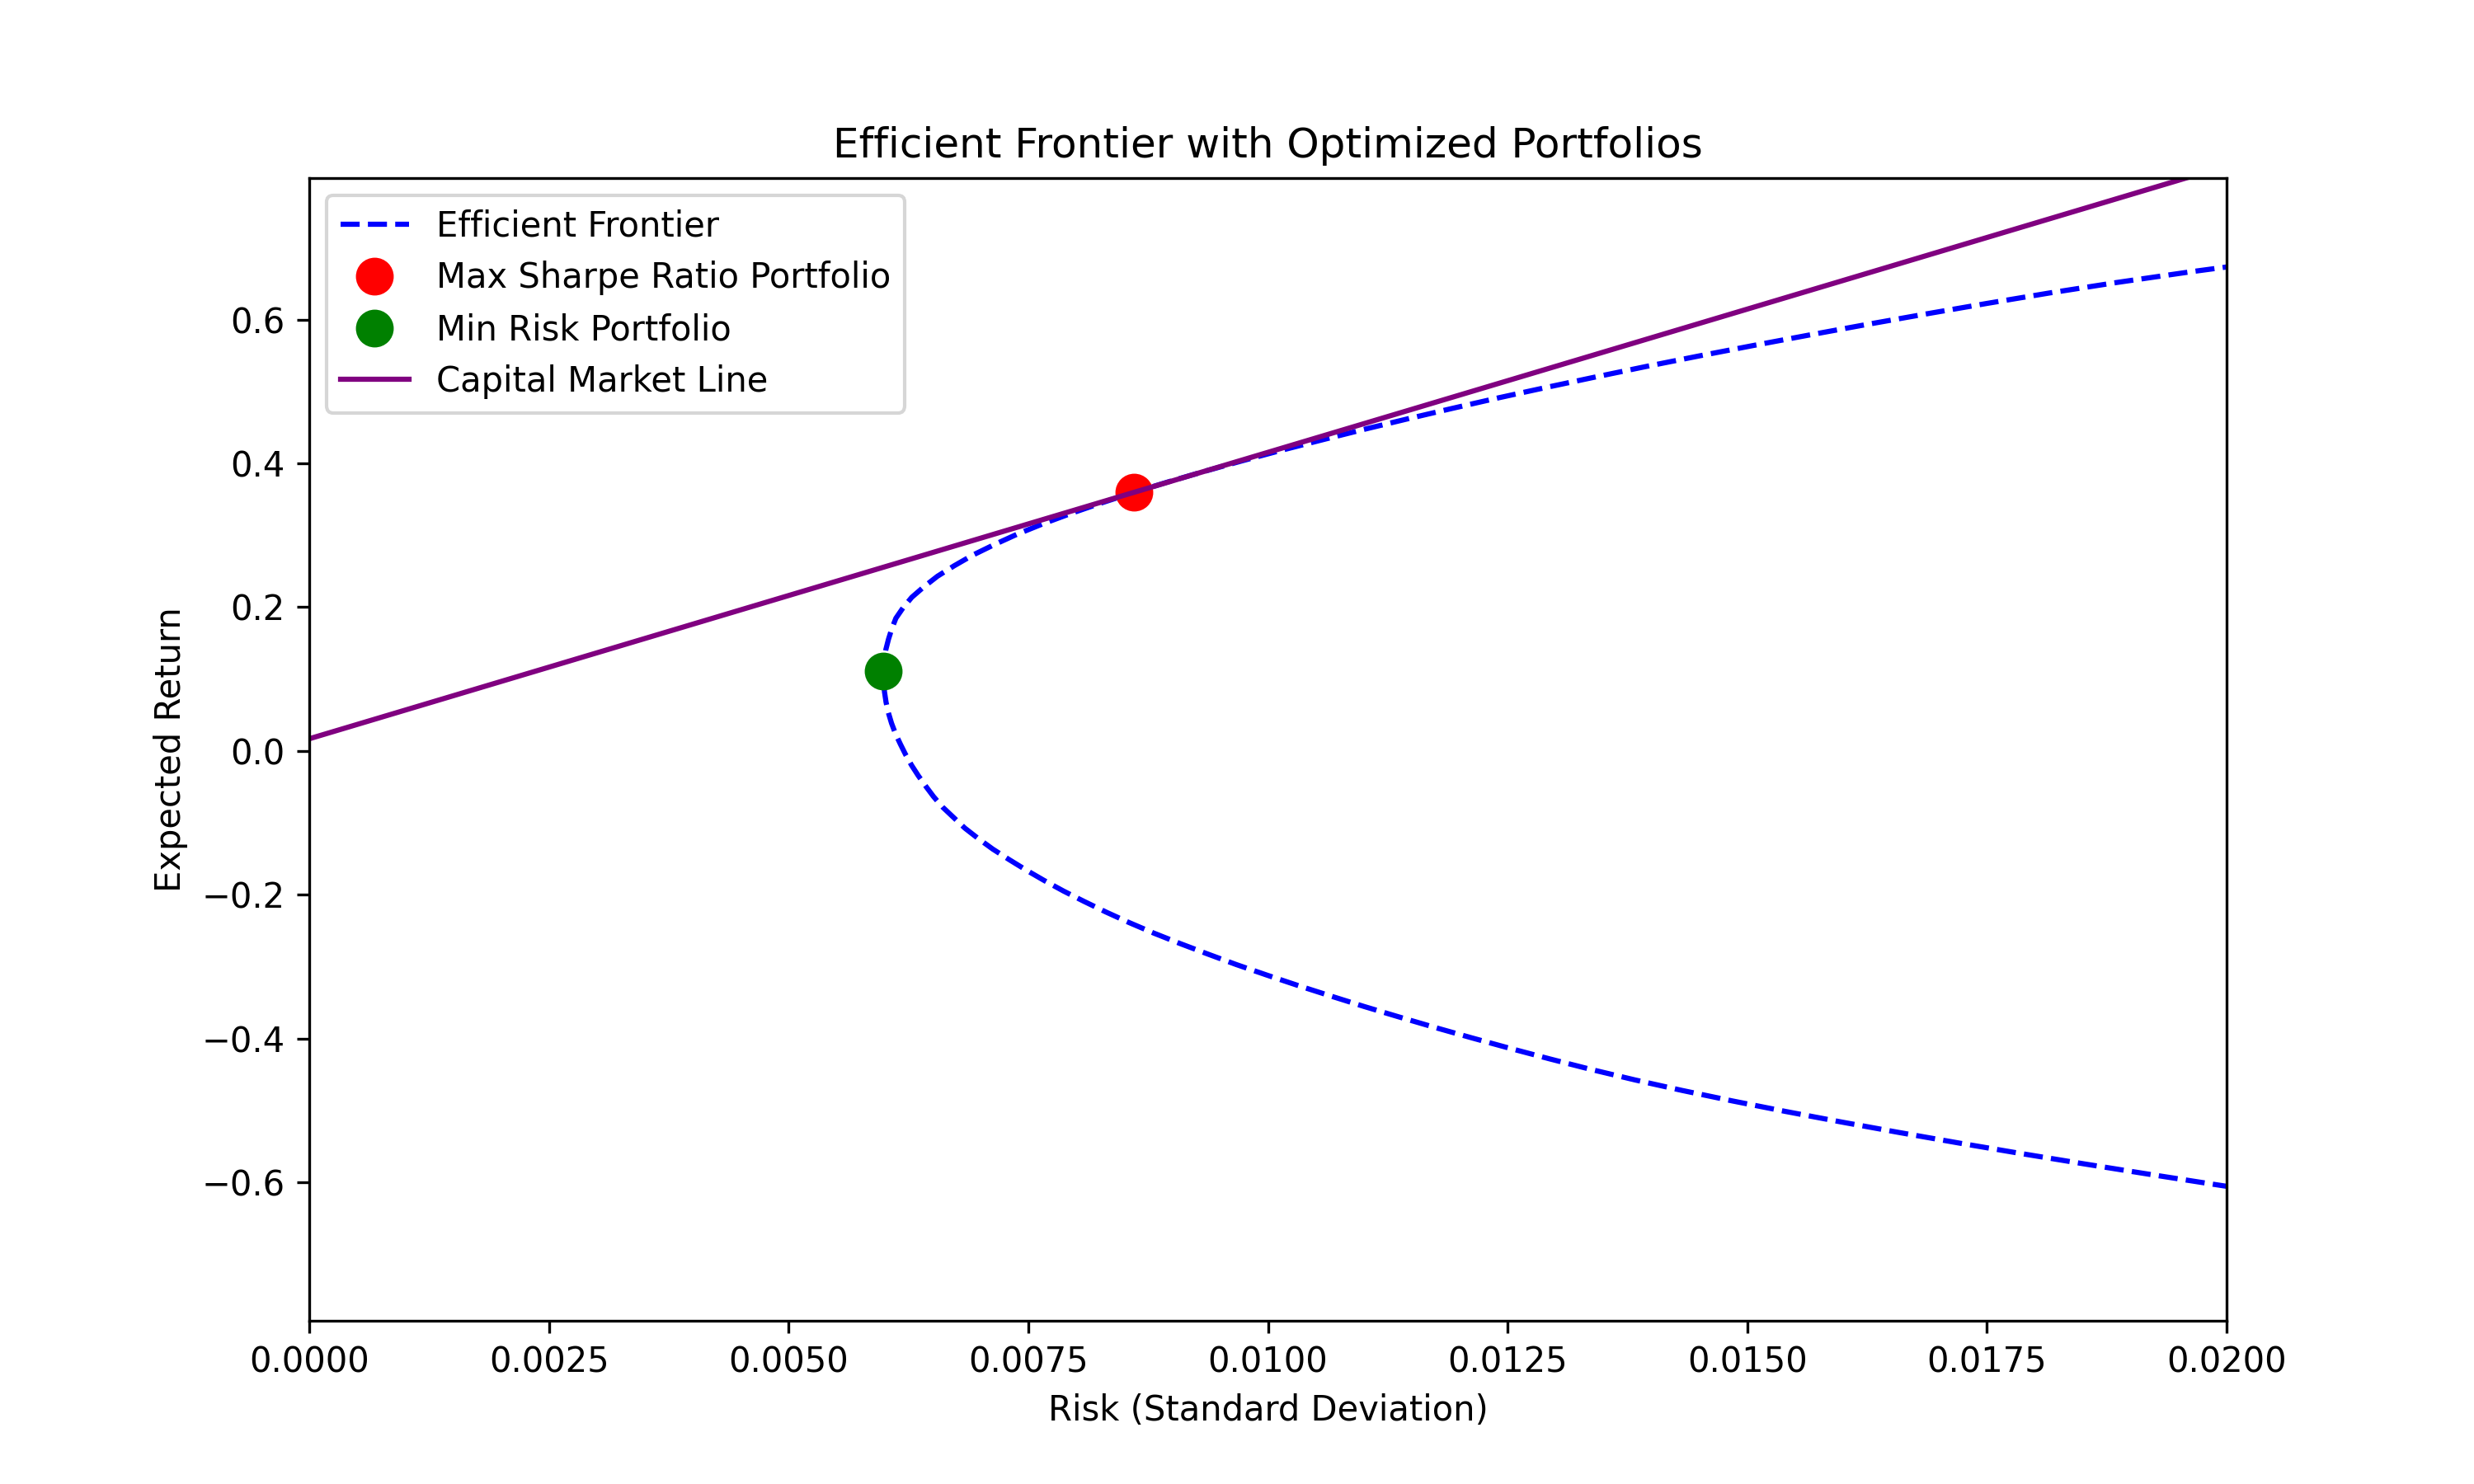
\includegraphics[width=0.8\textwidth]{figures/efficient_frontier.png}
    \caption{Plot showing the efficient frontier}
    \label{fig:efficient_frontier}
\end{figure}

\subsection{The Tangent Portfolio and The Capital Market Line}
% The tangent portfolio is the optimal risky portfolio, and it is the portfolio that has the highest Sharpe ratio.
% The capital market line is the line that connects the risk-free rate to the tangent portfolio.
% We now show the capital market line, and how to construct it.

The capital market line (CML) is the line that connects the risk-free rate to the tangent portfolio.
The tangent portfolio is the optimal risky portfolio, and it is the portfolio that has the highest Sharpe ratio.
The Sharpe ratio is given by:
\begin{equation}
    \label{eq:sharpe_ratio}
    S = \frac{E[R_p] - R_f}{\sigma_p}
\end{equation}
Where:
\begin{itemize}
    \item $S$ is the Sharpe ratio
    \item $E[R_p]$ is the expected return of the portfolio
    \item $R_f$ is the risk-free rate
    \item $\sigma_p$ is the standard deviation of the portfolio
\end{itemize}

The Sharpe ratio is a measure of the risk-adjusted return of a portfolio, and it is used to compare the performance of different portfolios.
The higher the Sharpe ratio, the better the portfolio's return per unit of risk.

Going back to Figure \ref{fig:efficient_frontier}, we can see that the CML is the line that connects the risk-free rate to the tangent portfolio.
It represents the set of all efficient portfolios that can be constructed by combining the risk-free asset with the tangent portfolio.
The line to the left of the tangent portfolio represents having a positive exposure to the risk-free asset, and the line to the right of the tangent portfolio represents having a negative exposure to the risk-free asset.
A negative exposure means taking out a loan to invest in the tangent portfolio.

The formula for the CML is given by some weight on the risk free rate, and some weight on the tangent portfolio:
\begin{equation}
    \label{eq:cml}
    E[R_p] = w_f R_f + w_t E[R_t]
\end{equation}
Where:
\begin{itemize}
    \item $E[R_p]$ is the expected return of the portfolio
    \item $w_f$ is the weight of the risk-free asset in the portfolio
    \item $R_f$ is the risk-free rate
    \item $w_t$ is the weight of the tangent portfolio in the portfolio
    \item $E[R_t]$ is the expected return of the tangent portfolio
\end{itemize}



  \section{Arbitrage Pricing Theory}
\label{sec:arbitrage_pricing_theory}
In this section we'll briefly discuss Arbitrage Pricing Theory (APT), and how it generalizes the Capital Asset Pricing Model (CAPM) as well as 
how Fama-Macbeth regressions can be used to estimate risk premia. The purpose of this section is not to be comprehensive,
but to briefly introduce concepts, as well as the code used when implementing portfolios in a systematic risk framework.

\subsection{Arbitrage Pricing Theory}
We've discussed \citet{fama_french_1993} and the Size and Value risk factors it proposes.
Throughout the article so far we've focused on one source of systematic risk, market risk.
From now on we will include the Size and Value factors in our equation for expected returns.

This multi-factor model has the form as per Equation~{\ref{eq:multi_factor}}. This is the model given by Arbitrage Pricing Theory (APT).

\begin{equation}
    \label{eq:multi_factor}
    E[R_i] = R_f + \beta_{i,m} \gamma_m + \beta_{i,s} \gamma_s + \beta_{i,v} \gamma_v
\end{equation}
Where:
\begin{itemize}
    \item $E[R_i]$ is the expected return of asset $i$
    \item $R_f$ is the risk-free rate
    \item $\beta_{i,m}$ is the asset's exposure to the market risk factor
    \item $\beta_{i,s}$ is the asset's exposure to the size risk factor
    \item $\beta_{i,v}$ is the asset's exposure to the value risk factor
    \item $\gamma_m$ is the market risk premium
    \item $\gamma_s$ is the size risk premium
    \item $\gamma_v$ is the value risk premium
\end{itemize}

For an asset $i$, the expected return is a function of its exposure to the market, size, and value risk factors, as represented by the Betas.
Risk premia are the expected returns of the systematic risk factors, and they are the same for all assets. Recall in the CAPM model, we were concerned only with
the market risk premium, now we have three risk premia.

Table ~\ref{tab:sample_asset_exposures} shows the exposures of a few sample assets to the market, size and value risk factors.

\begin{table}
    \centering
    \begin{tabular}{lccccc}
\toprule
Mkt-RF\_loading & SMB\_loading & HML\_loading & symbol \\
\midrule
1.113 & -0.251 & -0.379 & AAPL \\
0.983 & 0.140 & 0.582 & GE \\
0.804 & -0.147 & 0.335 & IBM \\
0.550 & -0.333 & 0.216 & KO \\
1.168 & -0.404 & -0.449 & MSFT \\
\bottomrule
\end{tabular}

    \caption{Sample assets and their exposures to the market, size and value risk factors}
    \label{tab:sample_asset_exposures}
\end{table}

We used to get the market risk premia by taking the average market return over our data period, but we will now introduce a way to get
the risk premia for the size and value factors.

\subsection{Fama-Macbeth Regressions}
Fama-Macbeth regressions are a two stage process that allows us to get the risk premia and factor sensitivities for a set of risk factors.

The first stage is a cross-sectional regression of the asset returns against the risk factors.
This gives us the factor sensitivities (betas) for each asset.
The second stage is a time-series regression of the factor sensitivities against the risk factors.
This gives us the risk premia for each factor at every time-step T.

Stage 1 is given by Equation~{\ref{eq:stage_1}}:
\begin{equation}
    \label{eq:stage_1}
    R_i = \alpha + \beta_{i,m} R_m + \beta_{i,s} R_s + \beta_{i,v} R_v + \epsilon
\end{equation}
Where:
\begin{itemize}
    \item $R_i$ is the return of asset $i$
    \item $\alpha$ is the intercept of the regression line
    \item $\beta_{i,m}$ is the asset's exposure to the market risk factor
    \item $\beta_{i,s}$ is the asset's exposure to the size risk factor
    \item $\beta_{i,v}$ is the asset's exposure to the value risk factor
    \item $R_m$ is the market return
    \item $R_s$ is the size return
    \item $R_v$ is the value return
    \item $\epsilon$ is the error term
\end{itemize}
The second stage is given by Equation~{\ref{eq:stage_2}}, where we're estimating the gammas using the betas from the first stage at every time period
t.
\begin{equation}
    \label{eq:stage_2}
    R_t = \gamma_{0,t} + \gamma_{m,t} \beta_{i,m} + \gamma_{s,t} \beta_{i,s} + \gamma_{v,t} \beta_{i,v} + \epsilon_t
\end{equation}
Where:
\begin{itemize}
    \item $R_t$ is the return of the portfolio at time $t$
    \item $\gamma_{0,t}$ is the intercept of the regression line at time $t$
    \item $\gamma_{m,t}$ is the market risk premium at time $t$
    \item $\gamma_{s,t}$ is the size risk premium at time $t$
    \item $\gamma_{v,t}$ is the value risk premium at time $t$
    \item $\epsilon_t$ is the error term at time $t$
\end{itemize}

We then take an average of the timeseries regression coefficients to get the risk premia for each factor.
These risk premia are also referred to as factor returns, since they are the expected returns of the risk factors.

If we take the cumulative sum of these risk premia coefficients, we can visually see the performance of the risk factors over time.
We can see this in figure \ref{fig:factor_returns}, where we plot the cumulative sum of the risk premia for the size and value factors.
\begin{figure}
    \centering
    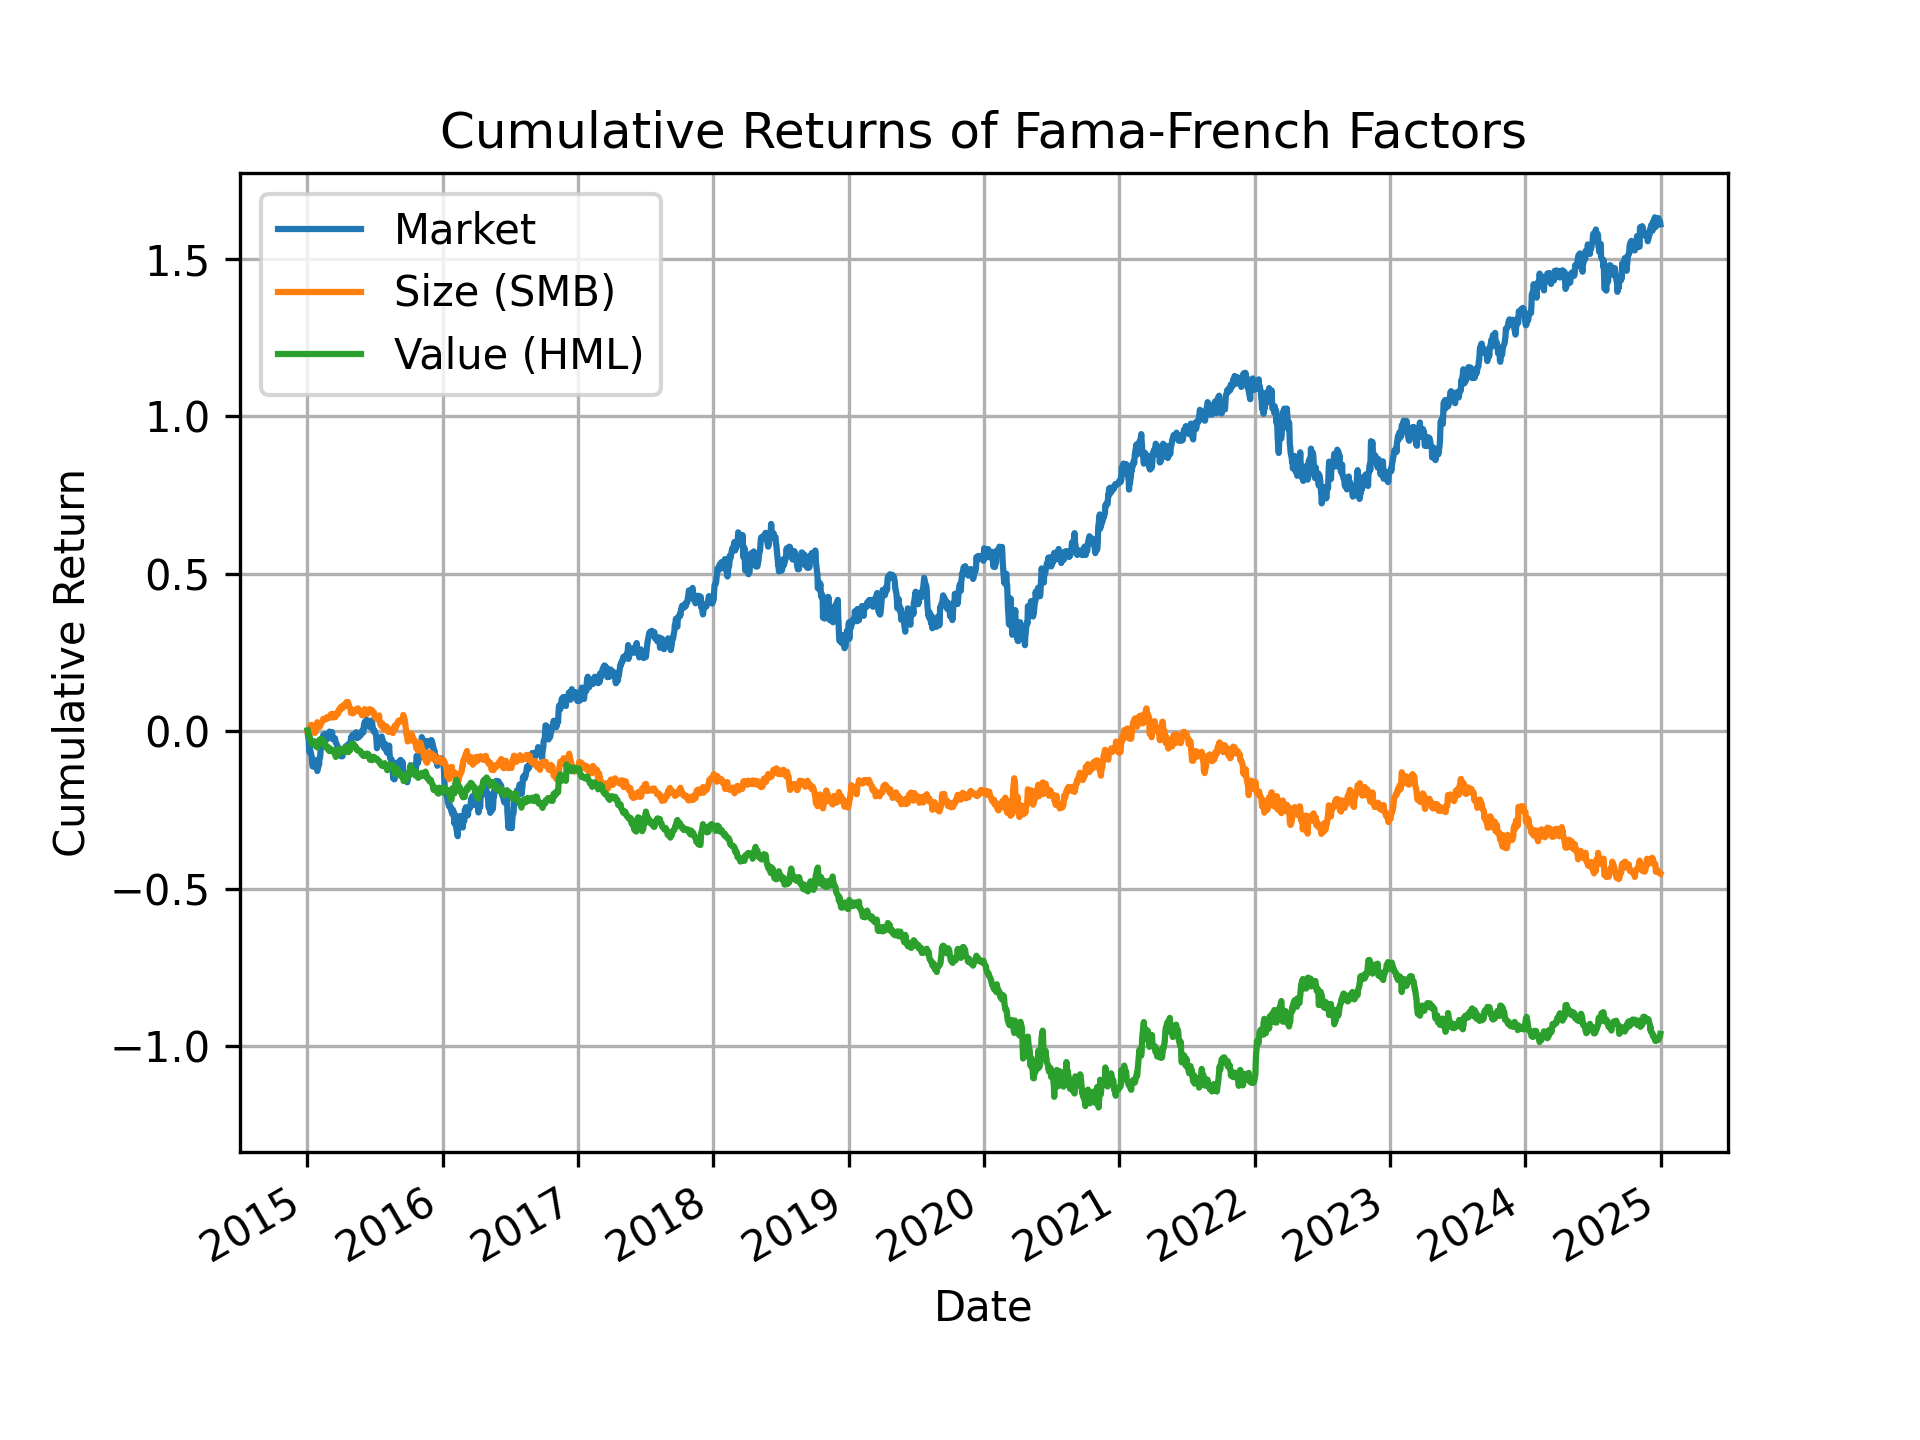
\includegraphics[width=0.8\textwidth]{../figs/factor_returns.png}
    \caption{Plot showing the cumulative sum of the risk premia for the market, size and value factors}
    \label{fig:factor_returns}
\end{figure}

We can take the averages of these coefficients to get the risk premia for each factor. The results are shown in table \ref{tab:expected_factor_returns}.
The negative premia we see on size and value factors come from a mix of using a small sample of assets, namely the bias from using the current constituents S\&P 500, our relatively short
lookback period of 10 years, and how value has underperformed in the ast few years.

We need two parts to construct portfolios, expected returns and risk.
We can get the expected returns from the Fama-Macbeth regressions, and we now, since we 
believe that returns are only a function of risk factors, we can use the covariance matrix of the risk factors to get the risk of the portfolio.
This greatly reduces the dimensionality of the problem, since we only need to estimate the covariance matrix of the risk factors, and not the covariance matrix of the assets.
Expected returns for APT portfolios are still weighted sums of the expected returns of the component assets. Risk is given slightly differently, as we are now using the covariance matrix of the risk factors, and not the covariance matrix of the assets.
The expected risk is given by Equation~{\ref{eq:apt_portfolio_risk}}:
\begin{equation}
    \label{eq:apt_portfolio_risk}
    \sigma_p^2 = w^T \Sigma w
\end{equation}
Where:
\begin{itemize}
    \item $\sigma_p^2$ is the variance of the portfolio
    \item $w$ is the vector of weights of the assets in the portfolio
    \item $\Sigma$ is the covariance matrix of the risk factors
\end{itemize}

Table~\ref{tab:apt_expected_returns} shows the expected returns for a few sample assets.
Table~\ref{tab:factor_cov_matrix} shows the covariance matrix of the risk factors.

\begin{table}
    \centering
    \vspace{1em}
    \begin{tabular}{lr}
\toprule
Factors & Expected Factor Returns \\
\midrule
Mkt-RF\_loading\_premium & 0.1612 \\
SMB\_loading\_premium & -0.0453 \\
HML\_loading\_premium & -0.0962 \\
\bottomrule
\end{tabular}

    \caption{Expected factor returns for the market, size and value factors}
    \label{tab:expected_factor_returns}
    \vspace{1em}
\end{table}
\begin{table}
    \centering
    \vspace{1em}
    \begin{tabular}{lr}
\toprule
symbol & expected\_return \\
\midrule
A & 0.17 \\
AAPL & 0.23 \\
ABBV & 0.10 \\
ABNB & 0.19 \\
ABT & 0.16 \\
\bottomrule
\end{tabular}

    \caption{Expected returns according to APT for a few sample assets}
    \label{tab:apt_expected_returns}
    \vspace{1em}
\end{table}
\begin{table}
    \centering
    \vspace{1em}
    \begin{tabular}{lrrr}
\toprule
 & Mkt-RF\_premium & SMB\_premium & HML\_premium \\
\midrule
Mkt-RF\_premium & 0.06 & 0.00 & -0.00 \\
SMB\_premium & 0.00 & 0.02 & 0.00 \\
HML\_premium & -0.00 & 0.00 & 0.02 \\
\bottomrule
\end{tabular}

    \caption{Factor covariance matrix for the market, size and value factors}
    \label{tab:factor_cov_matrix}
    \vspace{1em}
\end{table}


  \section{Conclusion}
\label{sec:conclusion}
\subsection{Summary}

\subsection{Limitations}

  \newpage
  \bibliographystyle{chicago}
  \bibliography{references}

  \newpage
  \section*{Appendix}
  \renewcommand{\thesection}{\Alph{section}}
  \setcounter{section}{0}
  \section{Appendix}
\label{sec:appendix}

In this appendix I provide evidence from Form 10-Ks for the numbers used in the DDM and DFCFM.

\begin{figure}[h!]
    \centering
    \includegraphics[width=0.7\textwidth]{../figs/amd-cash.png}
    \caption{Screenshot from \citet{amd_10_k} with Cash values}
    \label{amd_cash}
\end{figure}

\begin{figure}[h!]
    \centering
    \includegraphics[width=0.7\textwidth]{../figs/amd-common-stock.png}
    \caption{Screenshot from \citet{amd_10_k} with common stock values}
    \label{amd_cs}
\end{figure}

\begin{figure}[h!]
    \centering
    \includegraphics[width=0.7\textwidth]{../figs/amd-debt.png}
    \caption{Screenshot from \citet{amd_10_k} with AMD's debt}
    \label{amd_debt}
\end{figure}

\begin{figure}[h!]
    \centering
    \includegraphics[width=0.7\textwidth]{../figs/amd-eps.png}
    \caption{Screenshot from \citet{amd_10_k} with AMD's EPS}
    \label{amd_eps}
\end{figure}

\begin{figure}[h!]
    \centering
    \includegraphics[width=0.7\textwidth]{../figs/amd-income.png}
    \caption{Screenshot from \citet{amd_10_k} with AMD's Operating Income (EBIT)}
    \label{amd_ebit}
\end{figure}

\begin{figure}[h!]
    \centering
    \includegraphics[width=0.7\textwidth]{../figs/intc-debt.png}
    \caption{Screenshot from \citet{intel_10_k} with INTC's debt rates}
    \label{intc_debt_rate}
\end{figure}

\begin{figure}[h!]
    \centering
    \includegraphics[width=0.7\textwidth]{../figs/intc-earnings.png}
    \caption{Screenshot from \citet{intel_10_k} with INTC's Operating Income (EBIT) and EPS}
    \label{intc_ebit}
\end{figure}

\begin{figure}[h!]
    \centering
    \includegraphics[width=0.7\textwidth]{../figs/intc-cash.png}
    \caption{Screenshot from \citet{intel_10_k} with INTC's Cash and Debt}
    \label{intc_cash}
\end{figure}

\begin{figure}[h!]
    \centering
    \includegraphics[width=0.7\textwidth]{../figs/intc-common-stock.png}
    \caption{Screenshot from \citet{intel_10_k} with INTC's Shares Outstanding}
    \label{intc_cs}
\end{figure}

\begin{figure}[h!]
    \centering
    \includegraphics[width=0.7\textwidth]{../figs/intc-dividend.png}
    \caption{Screenshot from \citet{nasdaq_intc} with INTC's Dividend Payments}
    \label{intc_dividend}
\end{figure}

\begin{figure}[h!]
    \centering
    \includegraphics[width=0.7\textwidth]{../figs/tsm-dividend.png}
    \caption{Screenshot from \citet{nasdaq_tsm} with TSMC's Dividend Payments}
    \label{tsm_dividend}
\end{figure}

\begin{figure}[h!]
    \centering
    \includegraphics[width=0.7\textwidth]{../figs/tsmc-earnings.png}
    \caption{Screenshot from \citet{tsmc_10_k} with TSMC's EBIT, and EPS}
    \label{tsm_earnings}
\end{figure}

\begin{figure}[h!]
    \centering
    \includegraphics[width=0.7\textwidth]{../figs/tsmc-cash.png}
    \caption{Screenshot from \citet{tsmc_10_k} with TSMC's Cash Statements}
    \label{tsm_cash}
\end{figure}
\end{document}